% Created 2021-09-12 Sun 22:49
% Intended LaTeX compiler: xelatex
\documentclass[letterpaper]{article}
\usepackage{graphicx}
\usepackage{grffile}
\usepackage{longtable}
\usepackage{wrapfig}
\usepackage{rotating}
\usepackage[normalem]{ulem}
\usepackage{amsmath}
\usepackage{textcomp}
\usepackage{amssymb}
\usepackage{capt-of}
\usepackage{hyperref}
\usepackage[margin=1in]{geometry}
\usepackage{fontspec}
\usepackage{indentfirst}
\setmainfont[ItalicFont = LiberationSans-Italic, BoldFont = LiberationSans-Bold, BoldItalicFont = LiberationSans-BoldItalic]{LiberationSans}
\newfontfamily\NHLight[ItalicFont = LiberationSansNarrow-Italic, BoldFont       = LiberationSansNarrow-Bold, BoldItalicFont = LiberationSansNarrow-BoldItalic]{LiberationSansNarrow}
\newcommand\textrmlf[1]{{\NHLight#1}}
\newcommand\textitlf[1]{{\NHLight\itshape#1}}
\let\textbflf\textrm
\newcommand\textulf[1]{{\NHLight\bfseries#1}}
\newcommand\textuitlf[1]{{\NHLight\bfseries\itshape#1}}
\usepackage{fancyhdr}
\pagestyle{fancy}
\usepackage{titlesec}
\usepackage{titling}
\makeatletter
\lhead{\textbf{\@title}}
\makeatother
\rhead{\textrmlf{Compiled} \today}
\lfoot{\theauthor\ \textbullet \ \textbf{2021-2022}}
\cfoot{}
\rfoot{\textrmlf{Page} \thepage}
\titleformat{\section} {\Large} {\textrmlf{\thesection} {|}} {0.3em} {\textbf}
\titleformat{\subsection} {\large} {\textrmlf{\thesubsection} {|}} {0.2em} {\textbf}
\titleformat{\subsubsection} {\large} {\textrmlf{\thesubsubsection} {|}} {0.1em} {\textbf}
\setlength{\parskip}{0.45em}
\renewcommand\maketitle{}
\author{Houjun Liu}
\date{\today}
\title{Conductors and Equlibrium}
\hypersetup{
 pdfauthor={Houjun Liu},
 pdftitle={Conductors and Equlibrium},
 pdfkeywords={},
 pdfsubject={},
 pdfcreator={Emacs 28.0.50 (Org mode 9.4.4)}, 
 pdflang={English}}
\begin{document}

\maketitle


\section{Conductors at Equilibrium}
\label{sec:org28750dd}
If the charges on a conductor are \textbf{stationary}, no electron flow within
the conductor (so, it's \textbf{at equilibrium})\ldots{} This means that:

\begin{enumerate}
\item Net E-field \emph{in} the conducting material must be zero

\begin{itemize}
\item Because, uhh\ldots{}., the conductor is stationary, meaning no electron
flow
\item So, without electric flow, you know that there is no electrons
flowing, which means no electric field
\end{itemize}

\item Any electrons that would exist would cluster at the surface of the
conductor

\begin{itemize}
\item At equilibrium, the electrons would want to be as far away from
each other as possible, meaning that they would stick to the
surface --- to take advantage of the biggest
perimeter/circumference
\end{itemize}

\item At the surface of the conductor, if any E-\emph{field} is present, it must
be perpendicular to the surface

\begin{itemize}
\item If you have a horizontal component, the conductor would be, well,
\emph{conducting} electricity, making it rather not static. This
horizonal component will push electrons in the conductor around
until it doesn't exist
\item If the E-Field is perpendicular, because we are in the Physics
Vacuum, no charges will flow because it can't flow out of the
conductor into something else
\end{itemize}
\end{enumerate}

\begin{quote}
The net electric field inside a neutral conductor must be 0
equilibrium (at which point it is stationary)
\end{quote}

\begin{itemize}
\item A conductor at equlibirium would see electrons cluster at curves to
maintain perpendicularity of e-Fields

\begin{itemize}
\item Because there are more electrons towards the center and across the
conductor to push all electrons towards the extremities before
achieving equlibirium
\item If charges are evenly distributed instead of being concentrated on
sharper corners, the now-unbalanced electrons will create horizonal
components
\end{itemize}
\end{itemize}

\begin{figure}[htbp]
\centering
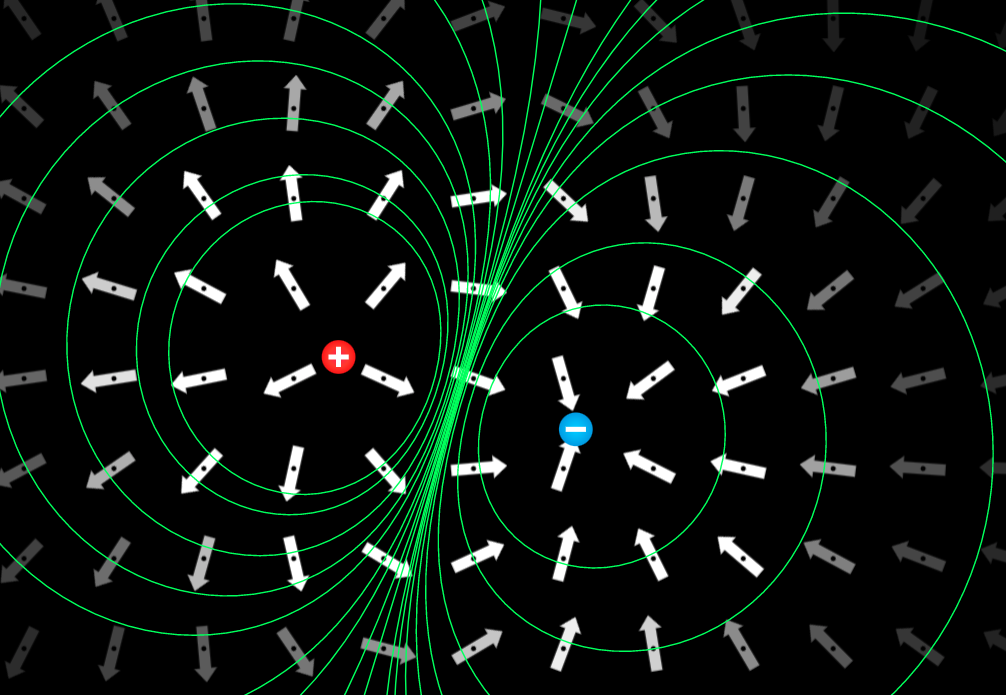
\includegraphics[width=.9\linewidth]{./2020PHYS201/20phys201srcPhETChargesAndFieldsConstantVoltage.png}
\caption{20phys201srcPhETChargesAndFieldsConstantVoltage.png}
\end{figure}

\begin{itemize}
\item PhET Exploration:

\begin{itemize}
\item r0N:
\href{KBe20phys201retFieldsVoltagePhET.org}{KBe20phys201retFieldsVoltagePhET}
\item 'Moka:
\href{KBhPHYS201PHETElectricFields.org}{KBhPHYS201PHETElectricFields}
\end{itemize}
\end{itemize}
\end{document}
